%
% drehung.tex
%
% (c) 2021 Prof Dr Andreas Müller, OST Ostschweizer Fachhochschule
%
\documentclass[tikz]{standalone}
\usepackage{times}
\usepackage{amsmath}
\usepackage{txfonts}
\usepackage[utf8]{inputenc}
\usepackage{graphics}
\usetikzlibrary{arrows,intersections,math}
\usepackage{ifthen}
\begin{document}

\definecolor{darkgreen}{rgb}{0,0.6,0}
\definecolor{darkred}{rgb}{0.6,0,0}

\newboolean{showgrid}
\setboolean{showgrid}{false}
\def\breite{7}
\def\hoehe{6}

\begin{tikzpicture}[>=latex,thick]

% Povray Bild
\node at (0,0) {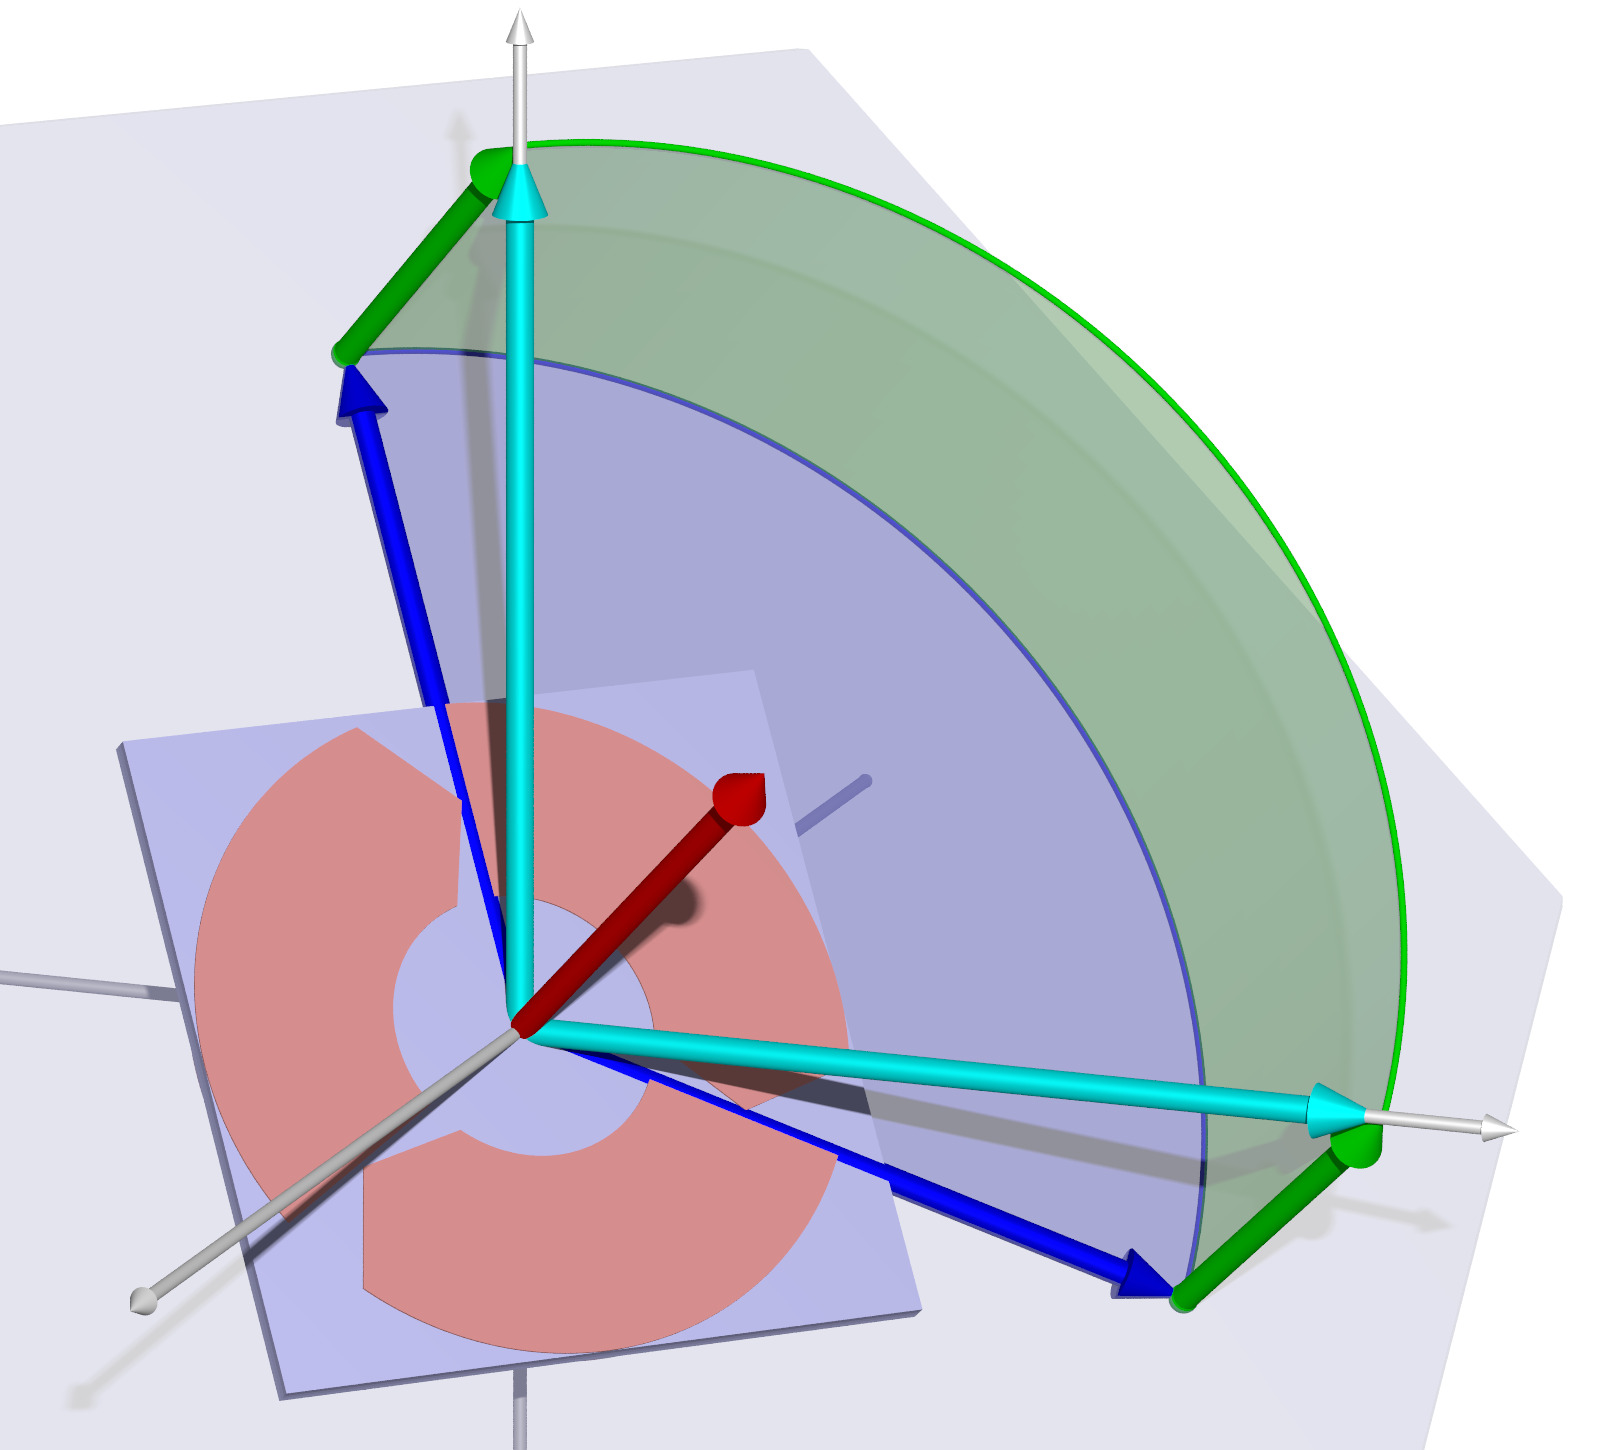
\includegraphics[width=13cm]{drehung.jpg}};

% Gitter
\ifthenelse{\boolean{showgrid}}{
\draw[step=0.1,line width=0.1pt] (-\breite,-\hoehe) grid (\breite, \hoehe);
\draw[step=0.5,line width=0.4pt] (-\breite,-\hoehe) grid (\breite, \hoehe);
\draw                            (-\breite,-\hoehe) grid (\breite, \hoehe);
\fill (0,0) circle[radius=0.05];
}{}

\node at (6.1,-3.3) {$a_1$};
\node at (-2.0,5.7) {$a_2$};
\node at (-5.7,-4.9) {$a_3$};

\node[color=white] at (-1.9,4.4) {$\boldsymbol{v}$};
\node[color=white] at (4.5,-2.7) {$\boldsymbol{v}''$};

\node[color=darkgreen] at (-3.3,4.4) {$\boldsymbol{v}_{\perp}$};
\node[color=darkgreen] at (4.2,-4.3) {$\boldsymbol{v}''_{\perp}$};

\node[color=blue] at (-3.7,1.5) {$\boldsymbol{v}_{\|}$};
\node[color=blue] at (1.9,-4.7) {$\boldsymbol{v}''_{\|}$};

\node[color=darkred] at (-1.6,-4.2) {$2\alpha=120^\circ$};
\node[color=darkred] at (-4.9,-0.6) {$\boldsymbol{q}$};

\end{tikzpicture}

\end{document}

